\documentclass[tikz, convert={convertexe=magick}, png]{standalone}

\usepackage{yquant, braket}
\yquantset{register/default name=$\ket{\reg_{\idx}}$}
\usetikzlibrary{fit, quotes}

\begin{document}
   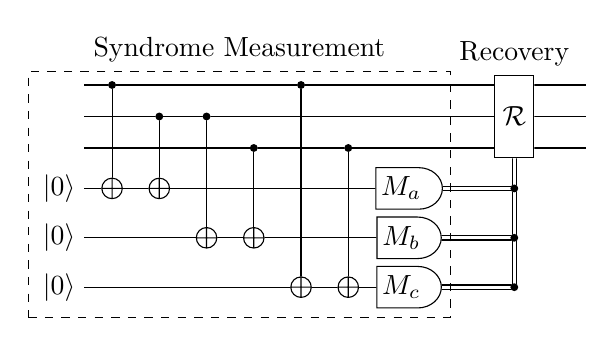
\begin{tikzpicture}
      \begin{yquant}
         qubit {} msg[3];
         [name=inits]
         qubit {$\ket0$} syndrome[3];
         
         [name=scnot0]
         cnot syndrome[0] | msg[0];
         cnot syndrome[0] | msg[1];
         cnot syndrome[1] | msg[1];
         cnot syndrome[1] | msg[2];
         cnot syndrome[2] | msg[0];
         cnot syndrome[2] | msg[2];
         [name=smeas]
         dmeter {$M_{\symbol{\numexpr`a+\idx}}$} syndrome;
         ["Recovery"]
         box {$\mathcal R$} (msg) | syndrome;
         discard syndrome;
      \end{yquant}
      \node[draw, dashed, fit=(inits-2) (scnot0-p0) (smeas-2), "Syndrome Measurement"] {};
   \end{tikzpicture}
\end{document}